In the previous section we explained why state-of-the-art resource allocation in cloud 
is sub-optimal for HPC workloads. This section will introduce our novel design that incorporates 
CPU and memory over-commitment for resource optimization. First, we start by introducing 
Virtual Throughput Clusters (VTC) with CPU over-commitment. Then, we continue to discuss the 
inclusion of memory over-commitment which is much more challenging. Lastly, we complete the design 
with dynamic VM migration, which mitigates potential 
performance penalties from resource over-commitment. 

\subsection{VTC with CPU over-commitment}
With a share-based CPU scheduler in the hypervisor, the allocation of CPU resource among VMs on a 
shared host does not entirely rely on the number of vCPUs, but also is affected by the configurable shares. 
This design change offers the CSPs or system admins the freedom to 
change VM vCPU numbers without worrying about impacting resource allocation. VTC takes advantage of this 
flexibility and configures each tenant with the same amount of virtual CPUs as the physical CPUs 
on a node. In this way, each tenant can get access to all the CPUs inside the node, and consequently, if one tenant 
is not consuming the entire quota, the free CPU cycles can be used by other tenant(s). 
This approach can be easily scaled to a cluster by repeating the configuration on every 
single node. Then, each tenant gets allocated a virtual cluster that consists of one VM per node. From the end user 
perspective, each tenant gets exclusive access to a dedicated cluster with isolation in security, fault, and even performance.  
Using the previous example of sharing four nodes between two tenants,  
VTC is illustrated in Figure~\ref{fig:vtc}. In the experiment section later, we will demonstrate  
support of upto 4 tenants simultaneously on a single physical cluster with 4X CPU over-commitment.

\begin{figure}[!t]
   \begin{center}
       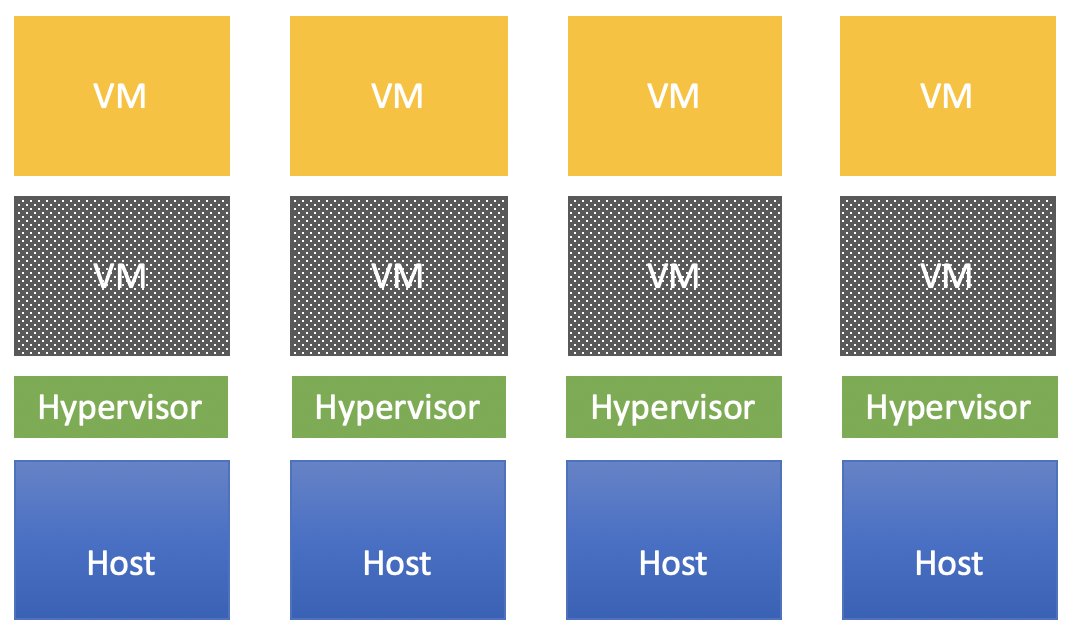
\includegraphics[width=\columnwidth]{Figures/allocation3}
   \end{center}
   \caption{Illustration of VTC on four nodes for two tenants.}
   \label{fig:vtc}
 \end{figure}

\subsection{Adding memory over-commitment}
Similar to CPU over-commitment, memory can be configured in a way that the combined VM memory can be 
larger than the physical memory capacity. It is impossible, however, that all VMs actively access all configured 
memory beyond the physical capacity. This is mainly due to performance considerations. TPS, ballooning, and 
compression all have no guarantee to reclaim memory in a timely manner, and if all these techniques fail, 
hypervisor swapping will occur to swap out guest OS memory to disks, rendering unacceptable performance to 
the HPC workloads. Two questions that we address through performance study in later section are: 1) whether memory over-commitment 
can be practical; 2) how far can we go with active memory usage under memory over-commitment.

\subsection{Dynamic VM migration}
It's very restricting that one can configure more VM memory but not able to consume all of them 
at the same time. This constraint applies to every node in the cluster because if memory is over stressed on any 
node, the progress of the whole workload is impacted. 
Fortunately, dynamic VM migration can be applied to relax the constraint~\cite{KannigaDevi2018,infrastructure2006resource}. 
It is often the case that nodes in an HPC cluster have varying memory load~\cite{gupta2013improving}. While some nodes have memory contentions 
between VMs, other nodes may have a decent amount of free memory. In such cases, VTC with memory over-commitment 
is much more promising because VMs can be dynamically migrated based on load changes to  
spread the memory load evenly across the physical cluster. Ideally, none of the nodes will experience sustained memory pressure as long as 
the total active memory does not exceed the physical cluster memory capacity. This essentially relaxes the previous 
per-node constraint to a constraint per cluster, which has much more room for memory pressure tolerance. 